%
% $RCSfile: two_tier_architecture.tex,v $
%
% Copyright (c) 2001-2004. Christian Heller. All rights reserved.
%
% No copying, altering, distribution or any other actions concerning this
% document, except after explicit permission by the author!
% At some later point in time, this document is planned to be put under
% the GNU FDL license. For now, _everything_ is _restricted_ by the author.
%
% http://www.cybop.net
% - Cybernetics Oriented Programming -
%
% http://www.resmedicinae.org
% - Information in Medicine -
%
% @author Christian Heller <christian.heller@tuxtax.de>
%

\subsection{Two Tier Architecture}
\label{two_tier_architecture_heading}

The proposed CYBOP communication architecture is currently implemented in form
of a \emph{Two-Tier} architecture (figure \ref{two_tier_architecture_figure}).

\begin{figure}[ht]
    \begin{center}
       \includegraphics[scale=0.4]{vector/two_tier_architecture.eps}
       \caption{Two Tier Architecture}
       \label{two_tier_architecture_figure}
    \end{center}
\end{figure}

It shows how two autarchic components (Application A and B) intercommunicate and
save their domain data in different ways. Each component fulfills a special task
and works as a client as well as a server. One can recognize the two patterns
\emph{DataMapper} and \emph{DTO}.\\
If a client requests some data from another component, the central object
\emph{DataTransferTranslator} collects all needed information from the
\emph{DomainModel} and encodes (packs) them into one \emph{DataTransferModel}.
Now, the \emph{Server} object can send this \emph{DTO} back to the requesting
client component. On the other side of the wire, the \emph{Client} object receives
the \emph{DTO}, a \emph{DataTransferTranslator} decodes (unpacks) the data and
writes them into the \emph{DomainModel}.\\
In this example, the two components are located on the same host. It is also
possible to distribute them. Therefore, each component is also able to communicate
with other components that are situated somewhere in the network. The arrows in
applications indicate the dependencies between the single architectural elements,
whereas the outside arrows show the communication between components and database
server.\\
All data storing operations are hidden in a special \emph{PersistenceTranslator}
like the one shown in figure \ref{two_tier_architecture_figure}, on the example
of a database. The SQL statements were placed in a separate package. If there is
the need for getting information from a database, the translator uses the statements
of the \emph{SQL Package} and maps data of the result set to the \emph{DomainModel}.

